\documentclass[11pt,twoside,a4paper]{report}
\setlength\parindent{0pt}
\usepackage{fullpage}
\usepackage{hyperref}
\hypersetup{
    colorlinks=true,
    linkcolor=black,
    urlcolor=blue,
}
\usepackage{mathtools}
\usepackage{booktabs}
\usepackage{ltablex}
\usepackage{amssymb}
\usepackage{graphicx}
\usepackage{tabularx}
\usepackage{gensymb}
\usepackage{pdfpages}
\usepackage{amsmath}
\usepackage{bm}
\usepackage{listings}
\usepackage{color}
\usepackage{float}
\usepackage[makeroom]{cancel}
\DeclareMathOperator{\csch}{csch}
\setlength\fboxrule{.3mm}
\DeclarePairedDelimiter\ceil{\lceil}{\rceil}
\DeclarePairedDelimiter\floor{\lfloor}{\rfloor}

\definecolor{dkgreen}{rgb}{0,0.6,0}
\definecolor{gray}{rgb}{0.5,0.5,0.5}
\definecolor{mauve}{rgb}{0.58,0,0.82}

\lstset{frame=tb,
  showstringspaces=false,
  columns=flexible,
  frame=none,
  basicstyle={\small\ttfamily},
  numbers=left,
  xleftmargin=.67cm,
  keywordstyle=\color{blue},
  commentstyle=\color{dkgreen},
  stringstyle=\color{mauve},
  breaklines=true,
  breakatwhitespace=true,
  tabsize=4
}

\def\dbar{{\mathchar'26\mkern-12mu d}}

\begin{document}

\tableofcontents


\section{Reflow Oven}

\subsection{Introduction}

\textit{Status: Functional}\newline

To do:
\begin{enumerate}
\item Review and understand microcontroller code.
\item Review and understand pc code.
\end{enumerate}

Building a homemade reflow oven will serve several benefits: (1) it will allow me to make PCBs in
the future with greater accuracy and less development time, and (2) it will give me a sense of how
to program, interact with and generally use microcontrollers to build embedded computers that have
less demanding performance constraints than is required when FPGAs are needed. FPGAs are often
overkill and many things can be done with a simple and cheap microcontroller. Additionally,
microcontrollers can often be used as a way to interface between an FPGA and a host computer.

\subsection{Materials \& Overview}

\subsubsection{Repository}
The repository for this project is at
\href{run:/home/matt/developer/reflow-controller}{/home/matt/developer/reflow-controller}. It
includes hardware design files as well microcontroller and host computer code. This project is taken
from Henrik Forsten, documented online
\href{http://hforsten.com/toaster-oven-reflow-controller.html}{here}.

\subsubsection{Hardware}
In addition to the materials specified by the hardware files, this also requires an ISP programmer
which is necessary to set fuse bits on the AVR microcontroller and also makes programming it
easier. The programmer can also be used in the future on any further AVR microcontroller. I am using
\href{https://www.sparkfun.com/products/9825}{this one}. The ISP uses an SPI interface to configure
the ATMega8U2 microcontroller. One of these pins is VCC that can be used to feed a 5V power supply
from the ISP to the reflow board. This feature can be toggled on and off using the power target
switch shown in Figure~\ref{fig:isp-power-switch}. Since that power line also connects to the
thermocouple ADC which can only support a max voltage of 4V, we must ensure that the power switch is
set to ``No Power'' before connecting the ISP to the AVR. In retrospect, it would have been much
better to route the header to VBUS instead of VCC which would have allowed us to use the ISP to
power the device.

\begin{figure}[h]
  \centering
  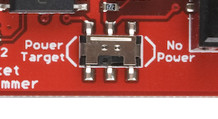
\includegraphics[width=0.4\textwidth]{data/isp-power-switch.jpg}
  \caption{The ISP power switch. ``Power Target'' will route 5V to the AVR and ``No Power'' will not
    route a signal to the AVR.}
  \label{fig:isp-power-switch}
\end{figure}

\subsubsection{Microcontroller Software}
Programming the AVR is done with \href{http://www.fourwalledcubicle.com/LUFA.php}{LUFA}, which in
turn depends on \href{https://www.nongnu.org/avrdude/}{AVRDUDE} and
\href{https://dfu-programmer.github.io/}{DFU-Programmer} as well as
\href{https://www.microchip.com/webdoc/AVRLibcReferenceManual/index.html}{AVR Libc}. The AVR code
uses a PID controller to control the operation of a solid state relay attached to the oven (PWM) and
attempts to converge the measured temperature to the target temperature at each time instant.

\subsubsection{Host Computer Software}
The host computer code is written in Python (don't forget to activate the VirtualENV environment
when using it) in the code repository. It listens at the serial port /dev/ttyACM0 and plots the
temperature readings from the AVR. It isn't strictly necessary, but is very useful especially since
the oven is too slow to match the temperature profile and some additional interactive steps must be
taken such as insulating the oven and opening the door during cool-down.

\subsection{Methods}

\subsubsection{Schematic}
The schematic for the controller is shown in Figure~\ref{fig:reflow-controller-sch}. The main
component on this board is an
\href{http://ww1.microchip.com/downloads/en/DeviceDoc/doc7799.pdf}{ATMega8u2 microcontroller} from
Atmel. The microcontroller has built-in support for USB communication and 8k bytes of flash
memory. It is clocked by an 8MHz external clock (which is necessary for USB functionality) and is
powered at 3.3V. In order to correctly power the device we externally supply the power in one of 2
ways: (1) connect a 5V supply to VBUS via the J5 connector, or (2) allow the host PC to provide the
5V over the USB connection. The second alternative should be preferred in most scenarios, since we
will generally plot the output of the PID controller to the host computer. In both instances, the 5V
power supply is downregulated via an onboard regulator,
\href{https://www.diodes.com/assets/Datasheets/AP2127.pdf}{AP2127K}, to the 3.3V used by the
microcontroller.\newline

\begin{figure}[h]
  \centering
  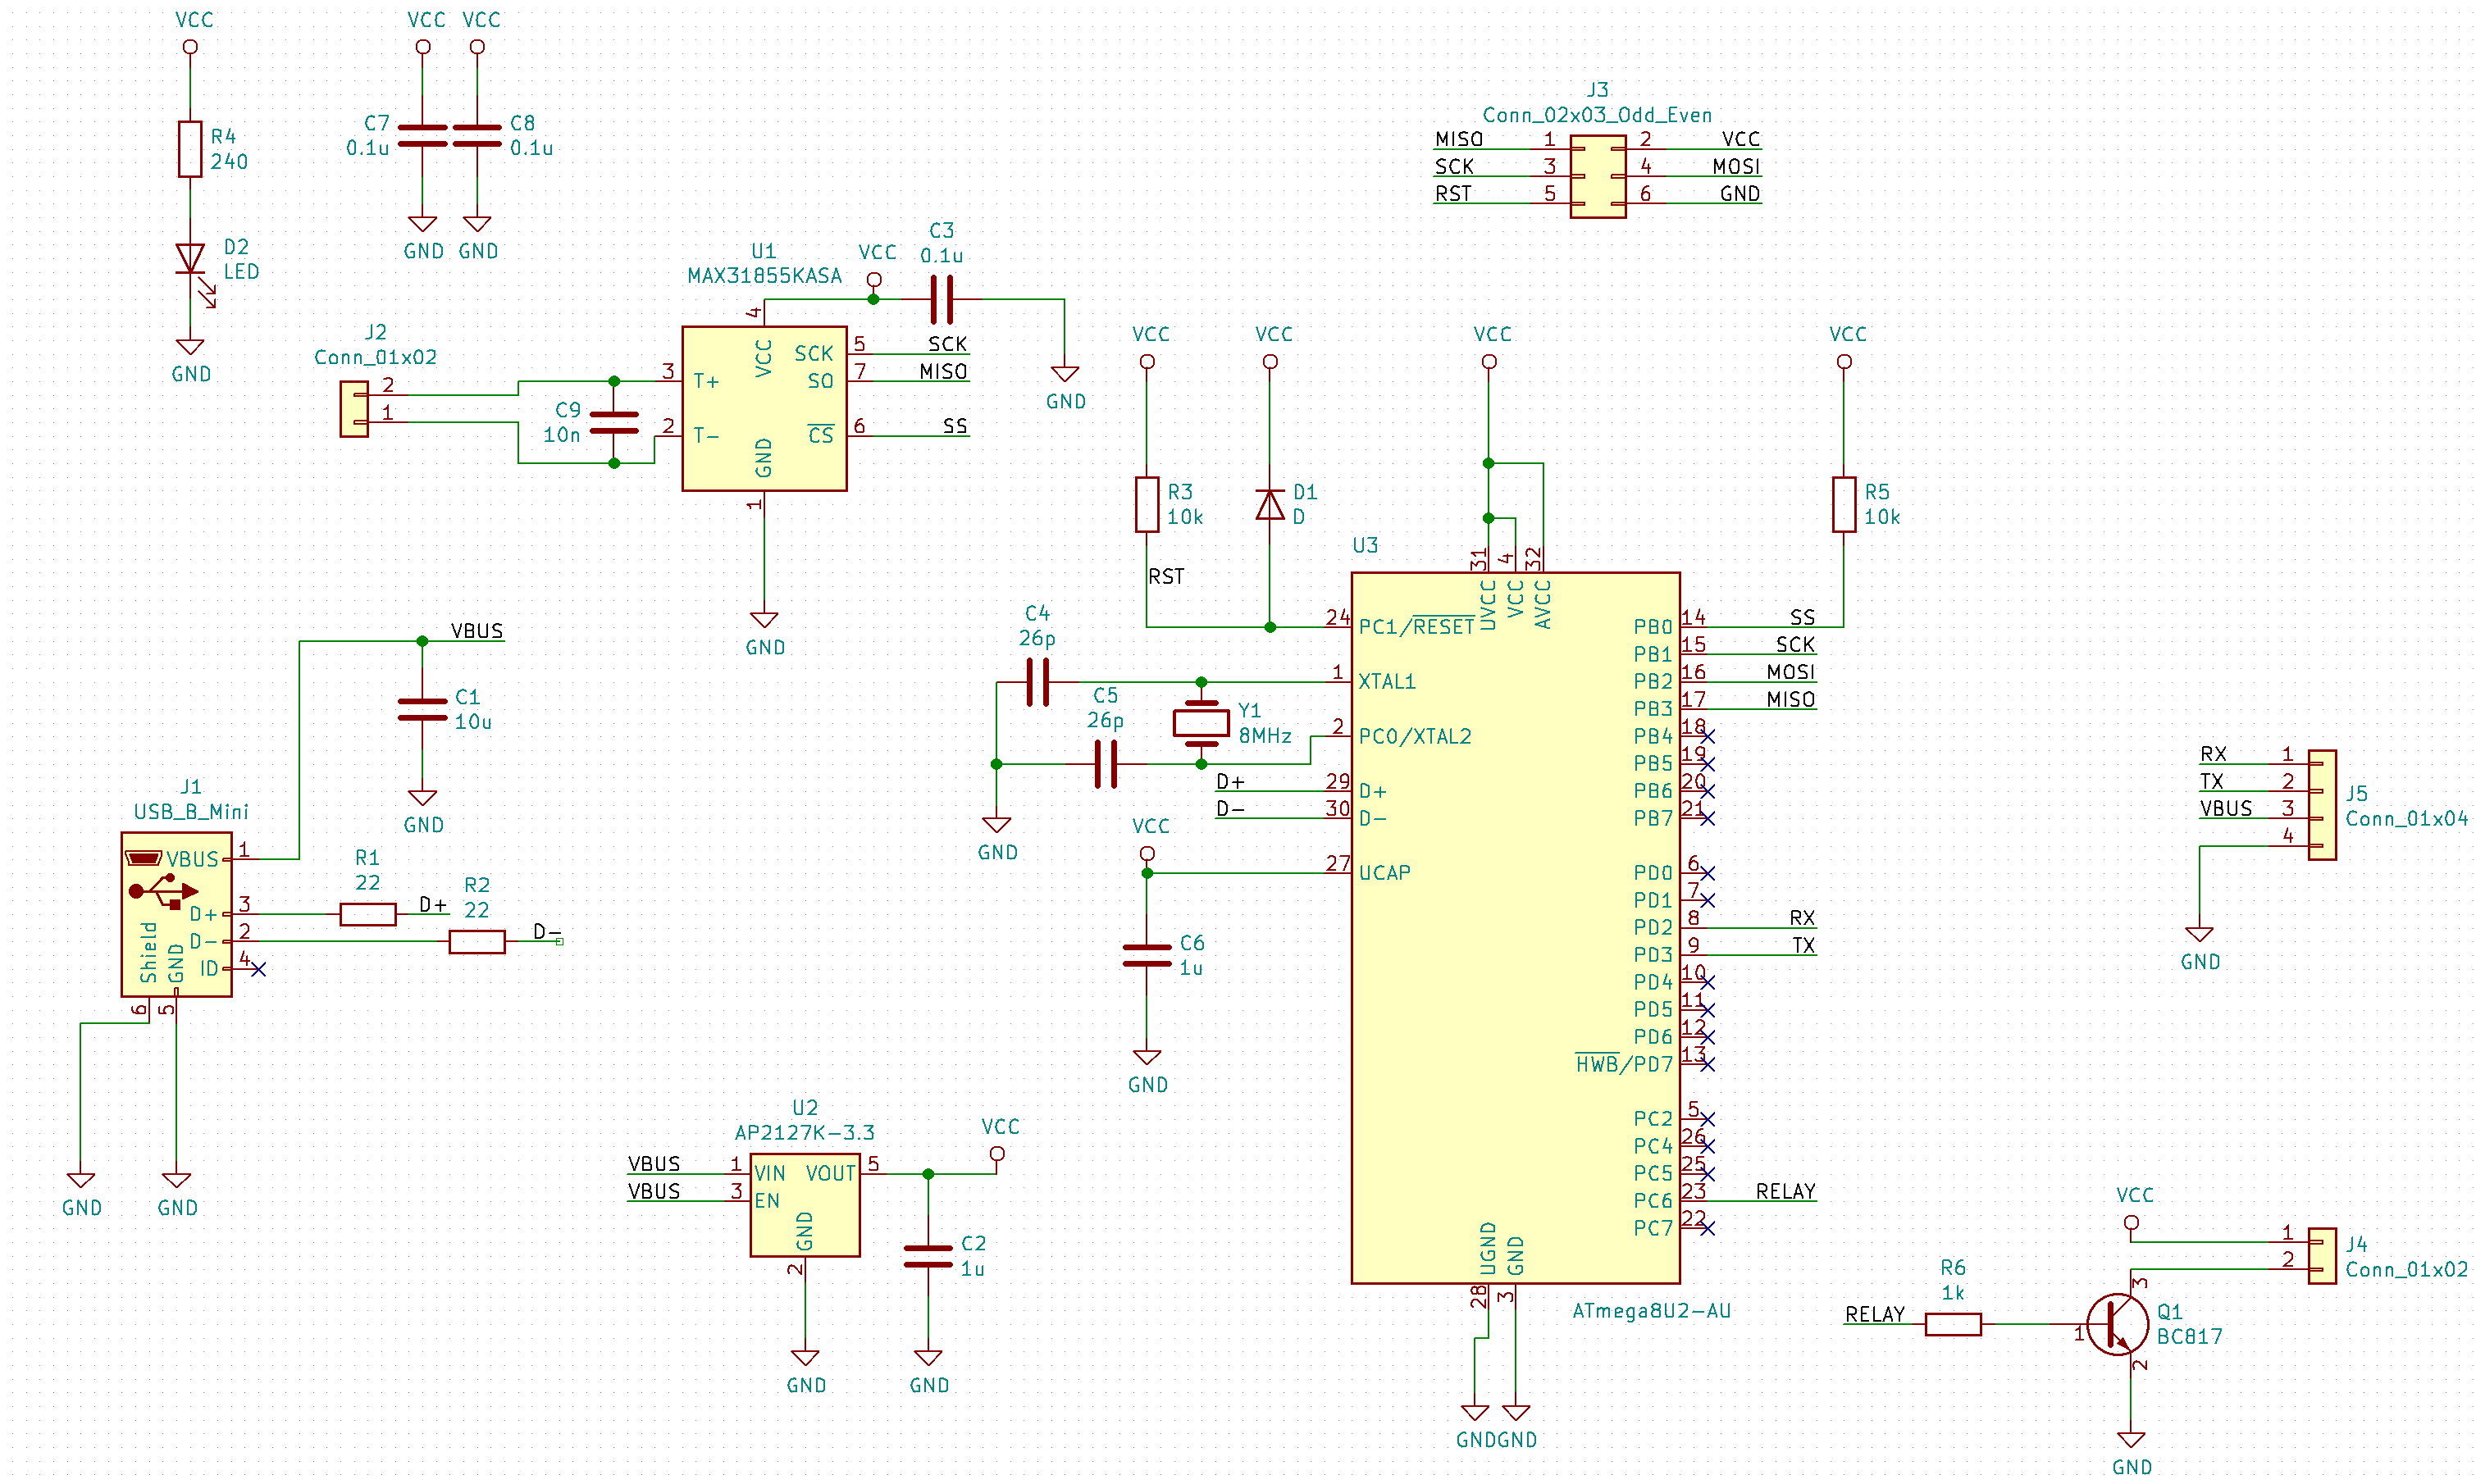
\includegraphics[width=\textwidth]{data/reflow-controller-sch.png}
  \caption{Reflow controller schematic.}
  \label{fig:reflow-controller-sch}
\end{figure}

The microcontroller is also connected to a thermocouple ADC,
\href{https://datasheets.maximintegrated.com/en/ds/MAX31855.pdf}{MAX31855}, via an SPI interface
that reads out the temperature from inside the oven. To communicate with the thermocouple ADC, the
ATMega8U2 pulls the SS line low and drives the SCK (note that the maximum clock frequency allowed by
the thermocouple ADC is 5MHz). It then reads out the temperature from the thermocouple ADC
synchronized by the SCK clock signal. The 10nF capacitor placed between the T+ and T- pins filters
noise between the thermocouple lines and was strongly recommended by the datasheet.\newline

The microcontroller then communicates via an open collector to the solid state relay, which switches
the power supply to the oven. The open collector line is attached to the PC6 pin of the
microcontroller, which is the channel A output compare pin (OC1A) of the microcontroller's built-in
PWM module. An internal waveform generator combinationally compares an internal timer/counter value
to the output compare register, OCR1A, and generates a variable frequency output (PWM) on the PC6
pin. The method of operation for this is shown in Figure~\ref{fig:fast-pwm}. A register (TCNT1)
counts up from 0 to a top value specified by another register (ICR1) at a frequency specified by a
prescaler. Once it reaches the top value it returns back to 0. When the value of TCNT1 matches the
value of a compare register (OCR1A) also set by us and reset periodically, OC1A will be set (since
we are using an open collector configuration, this will set it to 0) and when it matches the value
of ICR1, it will be cleared (set to 1 in our case). The diagram shows that in addition to being able
to update the value of OCR1A, we can update the top value, ICR1, which can be used to update the
period of the PWM signal. However, we won't use this in our configuration. The PWM frequency is
given by Equation~\ref{eq:pwm-freq}, which, for our configuration ($f_{\text{clk}}=8\text{MHz}$,
$N=256$ and $\text{TOP}=6250$), gives a frequency of 5Hz.

\begin{figure}[h]
  \centering
  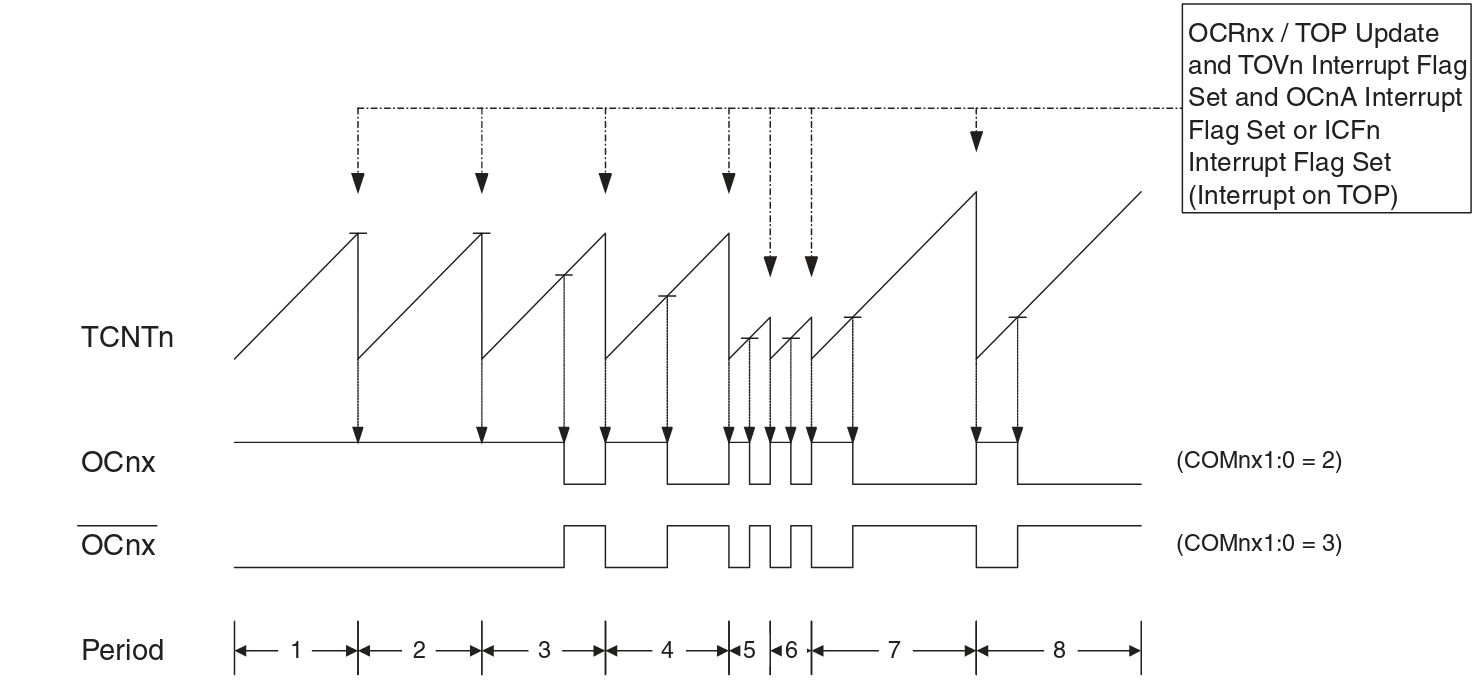
\includegraphics[width=0.75\textwidth]{data/fast-pwm.png}
  \caption{Fast PWM Mode timing diagram.}
  \label{fig:fast-pwm}
\end{figure}

\begin{equation}
  f_{\text{PWM}} = \frac{f_{\text{clk}}}{N \times (1 + \text{TOP})}
  \label{eq:pwm-freq}
\end{equation}

Finally, there is an additional connector (J3) that allows an ISP to configure the device.


\subsubsection{Microcontroller Software}
The microprocessor code depends heavily on the LUFA library and also includes several headers from
the AVR C standard library (\href{http://www.nongnu.org/avr-libc/}{Home Page} and
\href{http://www.nongnu.org/avr-libc/user-manual/index.html}{User Manual}). The LUFA USB.h header
file contains information about how to include the LUFA libraries and configure the ATMega8u2
microcontroller in order for it to enumerate and communicate correctly with a host computer. The
LUFA library allows several different configurations for the USB device, which correspond to
specific device drivers used by the host computer. The supported device classes are Android Open
Accessory, Audio 1.0, CDC-ACM, HID, MIDI, Mass Storage, Printer, RNDIS, and Still Image. Android
Open Accessory is for Android accessory devices, audio 1.0 is for audio devices such as microphones,
HID is for human interface devices such as keyboard and mice, MIDI is Musical Instrument Digital
Interface, Mass Storage is for USB storage devices, Printer is for printers, RNDIS is for network
devices attached to a USB bus, and Still Image is for digital cameras. Clearly, none of these are
relevant to our application. The only remaining device class is CDC-ACM, which can be used to
emulate serial ports over USB and transfer data between a host computer and a peripheral USB
device. This is the device class that we will use. It is worth noting that our microcontroller will
be acting as a device with a virtual serial port instead of as a device with a typical USB port,
even though the physical signals will still be transmitted over a USB cable and according to the USB
protocol. Although ACM seems to have been originally intended for modems and ISDNs, it is often used
for general data communication between a host computer and USB device, which matches our
application.\newline

LUFA defines a standard protocol that must be followed to correctly configure any device class. The
first step is to instantiate the ClassInfo struct (for our CDC device this is
\lstinline{USB_ClassInfo_CDC_Device_t}). The ClassInfo struct has two sections: a config section and
a state section. The config section must be fully specified in order to use the class driver. This
includes \lstinline{ControlInterfaceNumber}, \lstinline{DataINEndpoint},
\lstinline{DataOUTEndpoint}, and \lstinline{NotificationEndpoint}. This struct will be passed to
each of the driver's functions as the \lstinline{CDCInterfaceInfo} parameter. The code can be
adapted directly from the example provided by LUFA in the VirtualSerial demo. We must also copy the
LUFA directory from the root directory of the LUFA project and Config from the directory of the
VirtualSerial demo project to our microcontroller code directory.


\subsubsection{ATmega8U2 Configuration}
The ATmega8u2 AVR microcontroller comes preconfigured to use an internal oscillator rather than the
external crystal that I hooked up. This \href{http://www.engbedded.com/fusecalc/}{PalmAVR website}
can be used to set proper configurations and determine the corresponding fuse bits. It is important
not to use the external clock setting (external crystal or oscillator is fine) since that means you
intend to use an external clock (not soldered on the same PCB) and can be unrecoverable (or at least
difficult to recover from). The AVR came with the fuse bits
\lstinline{lfuse=0x5e hfuse=0xd9 efuse=0xf4} set. The fuse bits are described on page 247 of the
microcontroller datasheet. A fuse bit value of 0 indicates the corresponding fuse is programmed
whereas a fuse bit value of 1 indicates that fuse is not programmed. The clocking options are shown
in Table~\ref{tab:device-clocking-options}. \lstinline{efuse} stands for Extended Fuse Byte, which
controls the operation of brown-out detection and booting. \lstinline{hfuse} stands for Fuse High
Byte and controls the operation of several different things, none of which need to be
changed. \lstinline{lfuse} stands for Fuse Low Byte, which controls the operation of the clock
source and divide and is the only fuse byte that we need to reprogram. The default setting uses a
low power crystal oscillator, and divides the clock by 8, to generate a 1MHz clock.\footnote{The
  datasheet contains a contradiction. On page 29 it says that the device ships with the default
  clock source set to the internal RC oscillator. However, on page 248 it says that it ships with
  the clock source set to a low power crystal oscillator, which is correct.} We want to use the full
swing crystal oscillator and turn off the divide by 8 fuse. All other settings can be kept. This
corresponds to \lstinline{1101_0110} or \lstinline{0xd6}. \textbf{\{START INCOMPLETE\}} I have
previously set this value to \lstinline{0xbf}, which worked, although I think the other setting is
better. \textbf{\{END INCOMPLETE\}} This can be done with the command

\begin{lstlisting}[mathescape]
avrdude -c usbtiny -p atmega8u2 -U lfuse:w:0xd6:m -U hfuse:w:0xd9:m -U efuse:w:0xf4:m
\end{lstlisting}

\begin{center}
\begin{tabular}{l c}
  \textbf{Device Clocking Option} & \textbf{CKSEL3:0} \\
  \hline
  Low Power Crystal Oscillator & 1111 - 1000 \\
  Full Swing Crystal Oscillator & 0111 - 0110 \\
  Reserved & 0101 - 0100 \\
  Reserved & 0011 \\
  Calibrated Internal RC Oscillator & 0010 \\
  External Clock & 0000 \\
  Reserved & 0001 \\
  \label{tab:device-clocking-options}
\end{tabular}
\end{center}


\subsubsection{Host Computer Software}


\subsubsection{Soldering Attempts}
This \href{https://learn.adafruit.com/usbtinyisp/help}{Adafruit} article and this
\href{https://learn.sparkfun.com/tutorials/pocket-avr-programmer-hookup-guide/discuss}{Sparkfun}
article contain debugging information for a USBTiny device.\newline

My first attempt at soldering this device failed. These were the symptoms. When I plugged the device
directly into the USB port of my computer, the LED lit up and the ATMega8U2 microcontroller was
recognized by my computer. Additionally, I was able to erase the device memory with the command

\begin{lstlisting}[mathescape]
dfu-programmer atmega8u2 erase
\end{lstlisting}

This seems to indicate that at least part of the microcontroller was correctly soldered, and the
crystal and USB connector were correctly soldered. However, when I connected the ISP programmer to
the computer and connected the ISP header to the reflow controller, specifying ``No Power'', the LED
still lit up. Additionally, when I then connected a power supply across VBUS and GND, the current
between VBUS and GND was 0 (this may be normal; I forget whether the same thing occurred with the
board that worked). When the board was just connected to the 5V power supply, the current was about
60mA, which I believe was the same as the old board that worked. When I attempted to test the
connection with the board with the terminal command

\begin{lstlisting}[mathescape]
avrdude -c usbtiny -p atmega8u2
\end{lstlisting}

I got the error

\begin{lstlisting}[mathescape]
Could not find USB device 0x1781/0xc9f
\end{lstlisting}

which is apparently an error with USB3.x. Sure enough, when I tried the same thing with my older
Linux computer (with USB2.x ports), I got a new error

\begin{lstlisting}[mathescape]
initialization failed, rc=-1
\end{lstlisting}

which means that the computer was able to communicate with the ISP, but the ISP in turn was not able
to communicate with the board. This seems to either indicate that parts of the microcontroller were
incorrectly soldered, or the pin header was incorrectly soldered. I imagine that it was an issue
with the microcontroller since it seemed straightforward to solder the pin headers, and when the
microcontroller was first soldered there were a significant number of solder bridges that I had to
fix. Fixing the solder bridges both exposed the microcontroller to prolonged heat and potentially
lead to an insufficient amount of solder on the pins, or oxidation on the pins.\newline

The other changes that I made from the original design are an LED connected to between VCC and GND,
I got rid of the PTC connected to VBUS, and I added a diode for the power-on-reset connection. None
of these should adversely affect the operation of the board, including the LED, which should route
about 4.6mA of current through the diode. I see no reason why this should be bad for the operation
of the rest of the board.\newline

The way to solve this seems to be to improve the process of solder paste application to the
board. Every time I have applied solder paste it has been in between the pads in addition to on the
pads. I think I am applying way too much paste, which is consistent with the large number of solder
bridges that result after reflow (and that some components are not flat on the board). Follow the
directions in the soldering technique section to prevent this. Do not proceed with component
placement if there is solder between the pads. The other thing to do is to always connect 5V between
VBUS and GND \textbf{before} connecting the reflow board to the ISP. I'm not 100\% sure this will
make a difference, but it should ensure that the board gets the correct power supply.


\subsection{Discussion}

\subsection{Time Spent}


\end{document}